%Dokumententyp
\documentclass[a4paper]{article}


\usepackage[a4paper,left=2cm, right=3cm, top=2cm]{geometry}

%Kodierung
\usepackage[utf8]{inputenc}
\usepackage[T1]{fontenc}

%Grafiken einbinden
\usepackage{graphicx}
\usepackage{subfigure} 

%Position von Grafiken und Tabellen erzwingen:
\usepackage{float}

%URLs im Literaturverzeichnis
\usepackage{url}

\usepackage{amsmath}

%Vektoren einfacher angeben:
\newcommand{\vektor}[1]{\left( \begin{array}{c} #1 \end{array} \right) }


%Schriftart Arial:
% \usepackage{helvet}

%Figures with text around it:
\usepackage{wrapfig}

\usepackage{listings}

%seitennummern rechts:
% \usepackage{fancyhdr}
% \fancyhf{} % clear all header and footers
% \renewcommand{\headrulewidth}{0pt} % remove the header rule
% \rfoot{\thepage}
% \fancypagestyle{plain}{%redefining plain pagestyle
% \fancyhf %clear all headers and footers fields
% \fancyhead[R]{\thepage} %prints the page number on the right side of the header
% }

%Schriftart Times New Roman "like"
\usepackage{txfonts}

%Sprache
\usepackage[german]{babel}

%Checkmarks: (usage: \checkmark)
\usepackage{dingbat}

\usepackage{listings}
\usepackage{color}
\definecolor{javared}{rgb}{0.6,0,0} % for strings
\definecolor{javagreen}{rgb}{0.25,0.5,0.35} % comments
\definecolor{javapurple}{rgb}{0.5,0,0.35} % keywords
\definecolor{javadocblue}{rgb}{0.25,0.35,0.75} % javadoc
 
\lstset{language=Java,
basicstyle=\ttfamily,
keywordstyle=\color{javapurple}\bfseries,
stringstyle=\color{javared},
commentstyle=\color{javagreen},
morecomment=[s][\color{javadocblue}]{/**}{*/},
numbers=left,
numberstyle=\tiny\color{black},
stepnumber=1,
numbersep=5pt,
tabsize=4,
showspaces=false,
lineskip={-1.5pt},
showstringspaces=false}

%Tabellenextras
\usepackage{tabularx}

%Zeilenabstand 1.5
\linespread{1.5}
\usepackage{setspace}

%Figure Captions mit Fußnoten
\usepackage{footnote}
%\setlength{\parindent}{0pt} 


%itemize items richtig ausrichten (nicht links überlappen!)
% \setlist{leftmargin=0}

% %%%%TITELSEITE%%%%%%(
% \title{ Konzept und Implementierung\\ eines Systems zur \\Anforderung und Verwaltung von virtuellen privaten Clustern}
% \author{\textbf{\large Bachelorarbeit}}
% 
% \date{zur Erlangung des akademischen Grades Bachelor of Science an der Universität Paderborn im Fachbereich Informatik im Studiengang Bachelor Informatik}

% %%%%TITELSEITE%%%%%%)

% \pagestyle{fancy}
\begin{document}

\title{Algorithmische Geometrie - Sommersemester 2015\\
       5. Aufgabenblatt }
\author{Simon Koennecke und Felix Bröker}
\date{}
\maketitle

\section*{Aufgabe 1 - Voronoi-Diagramme von Strecken}

\section*{Aufgabe 2 - Fortune-Sweep}


\begin{figure} [!htb] 
	\subfigure[Schritt 1]{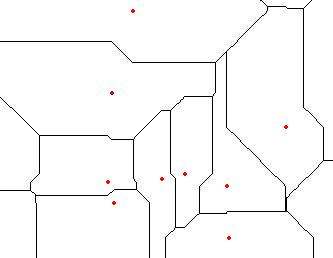
\includegraphics[width=0.5\textwidth]{01.png}} 
    \subfigure[Schritt 2]{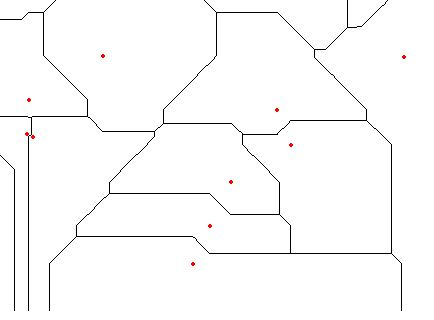
\includegraphics[width=0.5\textwidth]{02.png}} 
    \subfigure[Schritt 3]{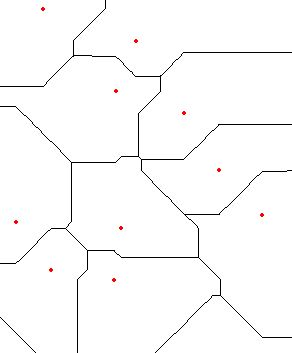
\includegraphics[width=0.5\textwidth]{03.png}} 
    \subfigure[Schritt 4]{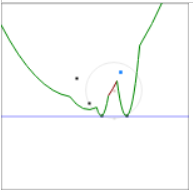
\includegraphics[width=0.5\textwidth]{04.png}} 
    \subfigure[Schritt 4]{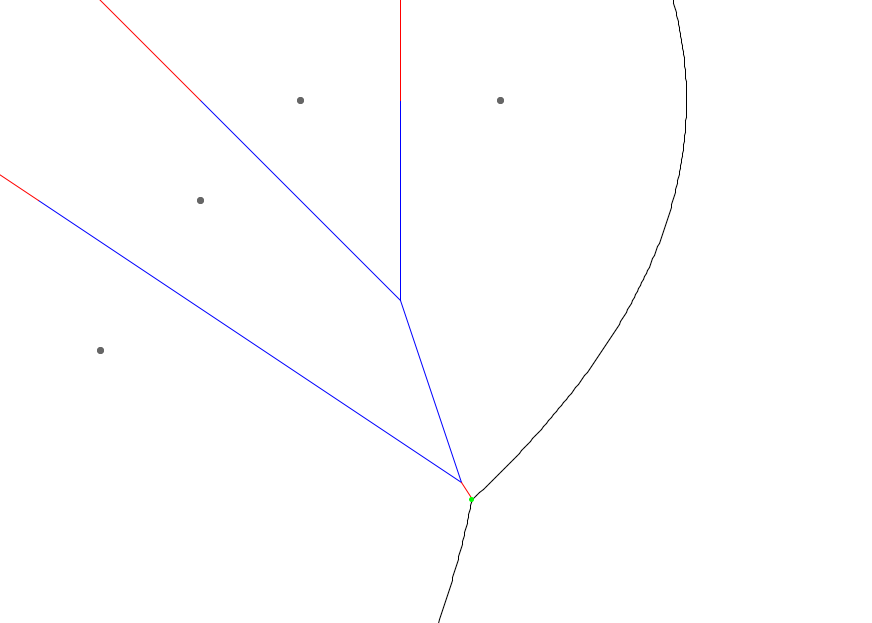
\includegraphics[width=0.5\textwidth]{05.png}} 
    \subfigure[Schritt 6]{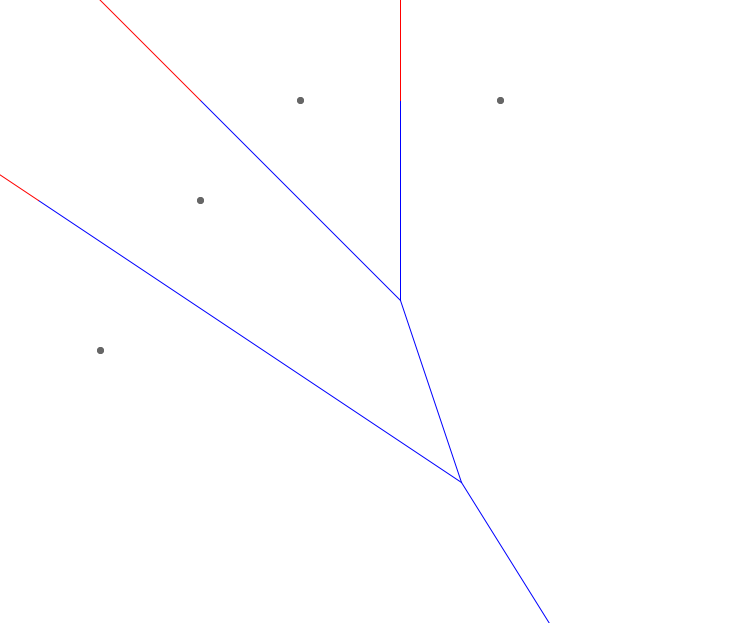
\includegraphics[width=0.5\textwidth]{06.png}} 
\end{figure} 

Quelle: http://www.raymondhill.net/voronoi/rhill-voronoi.html

Total number of sites processed: 4
Number of binary searches: 6
Avg number of iterations per binary search: 1.33
Number of parabolic cut calculations: 29 out of 69 total
Average beachline size: 4.00
Average circle event queue size: 0.75
Total number of cancelled circle events: 1 out of 3 total (33%)
Largest circle events queue size: 2 events
Number of destroyed edges (outside the viewport): 0 out of a total of 5 edges

Beachline is composed of 5 beach sections:
edge: none
xl=-Infinity, xr=53.3429, site={id:1, x:60, y:60}
edge: id=44, start=(x:95.0, y:55.0), end=(x:0.0, y:102.5)
xl=53.3429, xr=74.1682, site={id:2, x:70, y:80}
edge: id=45, start=(x:90.0, y:70.0), end=(x:10.0, y:150.0)
xl=74.1682, xr=90.0000, site={id:3, x:80, y:90}
edge: id=48, start=(x:90.0, y:70.0), end=(x:90.0, y:150.0)
xl=90.0000, xr=120.5831, site={id:4, x:100, y:90}
edge: id=46, start=(x:95.0, y:55.0), end=(x:136.3, y:0.0)
xl=120.5831, xr=Infinity, site={id:1, x:60, y:60}

\section*{Aufgabe 3 - Durchschnitt einfacher Polygone}





\end{document}
